\documentclass[11pt,a4paper]{article}
\usepackage[utf8]{inputenc}
\usepackage[T1]{fontenc}
\usepackage{amsmath}
\usepackage{amsfonts}
\usepackage{amssymb}
\usepackage[left=3.0cm, right=3.0cm, top=3.0cm, bottom=3.0cm]{geometry}
\usepackage{xcolor}
\usepackage{graphicx}
\usepackage{caption}
\usepackage{subcaption}

% include code listings
\usepackage{listings}

% Defining colors for syntax highlighting
\definecolor{codegreen}{rgb}{0,0.6,0}
\definecolor{codegray}{rgb}{0.5,0.5,0.5}
\definecolor{codepurple}{rgb}{0.58,0,0.82}
\definecolor{backcolour}{rgb}{0.95,0.95,0.92}

\lstdefinestyle{mystyle}{
	backgroundcolor=\color{backcolour},   
	commentstyle=\color{codegreen},
	keywordstyle=\color{magenta},
	numberstyle=\tiny\color{codegray},
	stringstyle=\color{codepurple},
	basicstyle=\ttfamily\footnotesize,
	breakatwhitespace=false,         
	breaklines=true,                 
	captionpos=b,                    
	keepspaces=true,                 
	numbers=left,                    
	numbersep=5pt,                  
	showspaces=false,                
	showstringspaces=false,
	showtabs=false,                  
	tabsize=2
}

\lstset{style=mystyle}
\captionsetup[lstlisting]{font={scriptsize}}

% header and footer
\usepackage{fancyhdr}
\pagestyle{fancy}
\fancyhf{}
\lhead{Michele Guadagnini}
\rhead{\today}
\lfoot{Ex 4 - Quantum Information and Computing 2020/2021}
\rfoot{Page \thepage}

\author{Michele Guadagnini - ID 1230663}
\title{\textbf{Exercise 4 \\ Automated runs, plots and fits}}
\date{\today}

%File names must include your name, exercise number and codewords REPORT, and CODE.
%Example: Ex2-Rossi-REPORT.pdf
%The maximum length of the report is five pages
\begin{document}
\maketitle

\vspace{20pt}
\begin{abstract}
	This exercise is about using a \textit{FORTRAN} compiled executable in a \textit{Python} script to run it multiple times with different parameters. Then, the data produced are plotted and fitted automatically by using a \textit{gnuplot} script.
\end{abstract}

\section{Theory} %Explain briefly the theory you have based your solution on.

The execution time of a certain program is the time spent by the CPU while completing the task.
It depends on the specific hardware on which it is executed (processor speed, disk and memory speed). Also, it can make use of these resources with more or less efficiency.
Optimizations to achieve better efficiencies can be applied on the source code and, for compiled languages, at compile time.
\textit{FORTRAN} in particular provides many different optimization levels; the ones used in this assignment are:
\begin{itemize}
	\item "-O0": it applies no optimization at compile time (default);
	\item "-O2": it activate some optimizations and make the compiler take longer to finish;
	\item "-Ofast": it activates all the optimizations.
\end{itemize}

In this exercise the execution time of a matrix multiplication is measured for three different methods and by scaling up the size of the matrices (for simplicity in this case matrices are assumed to be square).
A good model to fit the curves obtained from these data can be a power law model, that can be transformed into a linear fit by taking the logarithm of both \textit{x} and \textit{y} values.


\section{Code Development} %Introduce strategies, tests, and report debugging problems, compilations options

\subsection{Design and Implementation}
The implementation started from modifying the \textit{FORTRAN} code from the previous assignment by creating the function that reads the desired matrix size from a file, implementing it in the \textit{LoopMultiply} module. It also checks the size to be a positive integer number, otherwise it prints an error message.

%This function's code is showed in the following listing:
%\lstinputlisting[language=FORTRAN, firstline=46, lastline=70, firstnumber=46, caption=ReadSizeFromFile function.]{Ex4-Guadagnini-LoopMultiply-CODE.f90}

Matrices are set to be square with numbers between $0$ and $1$ of \textit{DOUBLE PRECISION} type.
The name of the file containing the matrix size is passed to the program as a command argument together with the output file names for the three different methods and the optional debug flag.

Then the subroutine to save the results has been implemented (\textit{WriteExecTimeToFile}). It receives as input the \textit{unit} number of the output file, the matrix size and the execution time measured and it writes them in the file side by side.

Also a subroutine called \textit{CatchError} has been added and used in the program alongside the \textit{CheckPoint} one in the module \textit{Debugger}. 
This new subroutine prints a message when an error occurs and, if the error is set to be a \textit{fatal} error through the dedicated logical variable, it prints the same message also in a file in order to expose the error to an eventual external script and stops the execution.

Once finished the implementation of the program performing the multiplication, a script to call it repeatedly with different arguments has been created using Python.
The script is called \textit{Ex4-Guadagnini-PyScript-CODE.py} and its main part is reported in the following listing:
\lstinputlisting[language=python, firstline=24, lastline=63, firstnumber=24, caption=Multi-Run python script.]{Ex4-Guadagnini-PyScript-CODE.py}

It starts by resetting all the output files, then it writes the matrix size in \textit{MatrixSize.txt} starting from $50$ until $2000$ with steps of $50$.
Since the program has been compiled with three different optimization flags (as explained above), the script runs all the three executable using a \textit{for} loop passing the respective output files.
If the multiplication program encounters an error, the python script is aware of this by looking at the size of the error file and prints a message while stopping the execution.

The last part of the exercise was to use \textit{gnuplot} to plot the obtained curves and fit them automatically through a python script.
The set of instruction used for the fit are in the file \textit{AutoFit.gnu} that is passed as argument when running \textit{gnuplot} from the python script \textit{Ex4-Guadagnini-AutoFit.py}. 
The script simply lists all the ".txt" files in the current folder and pass them one by one to \textit{gnuplot} that execute the fit, and changes the name of the \textit{fit.log} file. 
To perform a linear fit, gnuplot takes the logarithm of both the matrix size and the timings and applies the linear model:
\begin{equation*}
F(x) = ax + b
\end{equation*}
The following listing reports the gnuplot instruction set for the fits:
\lstinputlisting[language=gnuplot, caption=gnuplot script performing a fit.]{Data/AutoFit.gnu}

\subsection{Debug and Test}
The multiplication program has been tested before the use in the script by compiling and calling it in the terminal with the command:
\begin{lstlisting}[language=BASH, numbers=none]
gfortran *CODE.f90 -o MatrixTest.x
./MatrixTest.x MatrixSize.txt 1stLoop.txt 2ndLoop.txt MATMUL.txt
\end{lstlisting}

To test the error handling capabilities of the code, the python script has been temporary modified to write as matrix size a negative float number and also to not create the file at all. 
As expected, the FORTRAN executable encountered an error since it was not able to properly read the matrix size or the file containing it; through the function \textit{CatchError} a message was printed on screen and in this case also in the dedicated file \textit{FATAL\_ERRORS.txt}. 
By checking that this file was no more empty, also the python script stopped and printed the coded message, suggesting to look on that file for details on the error.

\section{Results} %Present data and explain your results.

In Figures \ref{fig:methods} are presented the pictures of the curves obtained for different methods and optimizations. The scale on the $y$ axis has been set to "log" since values space between $7$ orders of magnitude.
\begin{figure}
	\centering
	\begin{subfigure}{0.47\textwidth}
		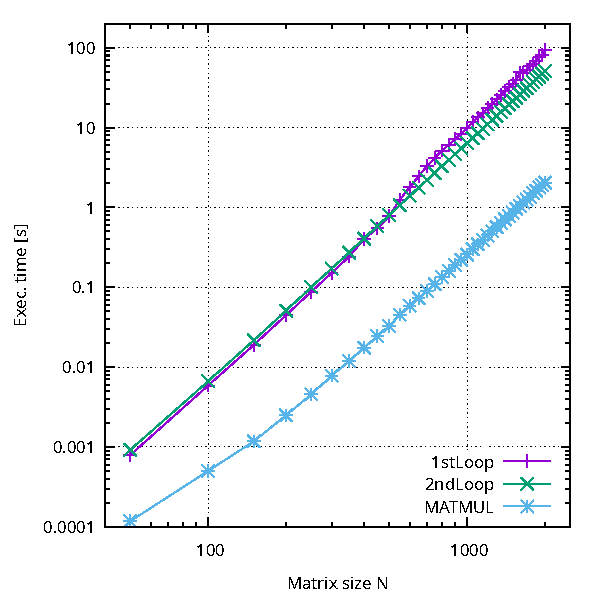
\includegraphics[width=1\linewidth]{Data/MethodsO0}
		\caption{All three methods with -O0 flag}
    	\label{fig:methodsO0}
	\end{subfigure}%
	\hfill
	\begin{subfigure}{0.47\textwidth}
		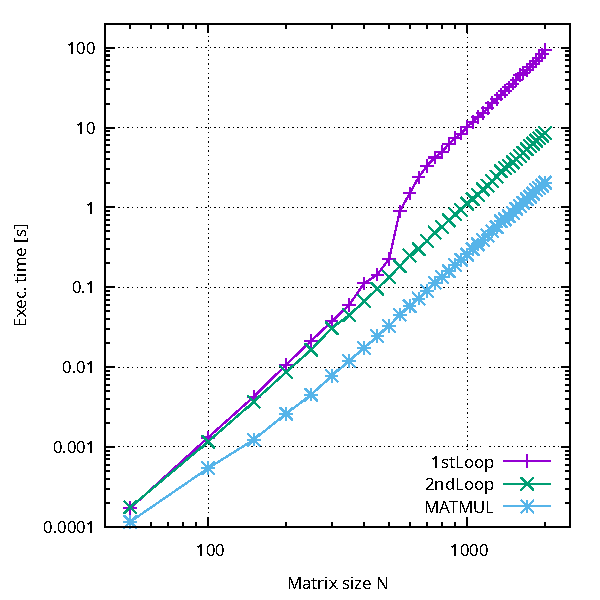
\includegraphics[width=1\linewidth]{Data/MethodsO2}
		\caption{All three methods with -O2 flag}
		\label{fig:methodsO2}
	\end{subfigure}
	\begin{subfigure}{0.47\textwidth}
		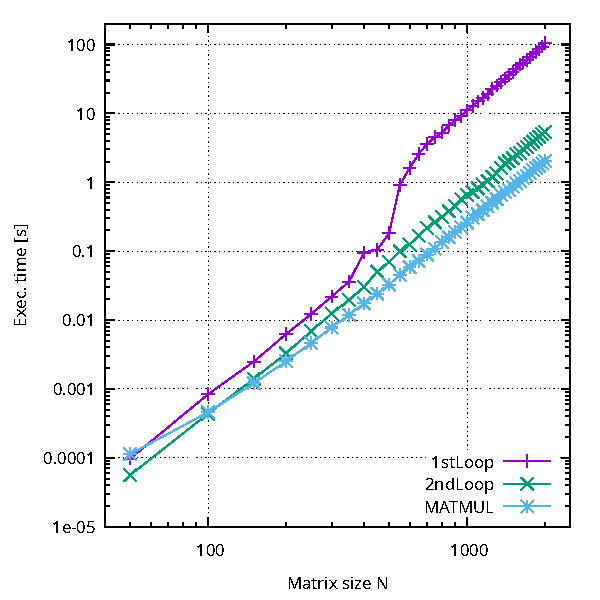
\includegraphics[width=1\linewidth]{Data/MethodsOfast}
		\caption{All three methods with -Ofast flag}
		\label{fig:methodsOfast}
	\end{subfigure}
	\caption{Time scaling for different methods and optimizations}
	\label{fig:methods}
\end{figure}
Comparing the figures it can be seen that the method that mostly benefits from optimization flags is \textit{2ndLoop}, while \textit{1stLoop} only have a small improvement until size $500$ and \textit{MATMUL} seems to be not sensitive to optimization flags.

Figure \ref{fig:fitso2} reports the fits of the timings for the three methods compiled with \textit{-O2} flag. In particular Figure \ref{fig:fit1stloopo2} shows a bad fit due to the jump in execution time for \textit{1stLoop} method around matrix size of $500$ ($Log_{10}(500) \approx 2.7$). The other two fits (Figures \ref{fig:fit2ndloopo2} and \ref{fig:fitMATMULo2}) seems to be more accurate.

\begin{figure}[t]
	\centering
	\begin{subfigure}{0.47\textwidth}
		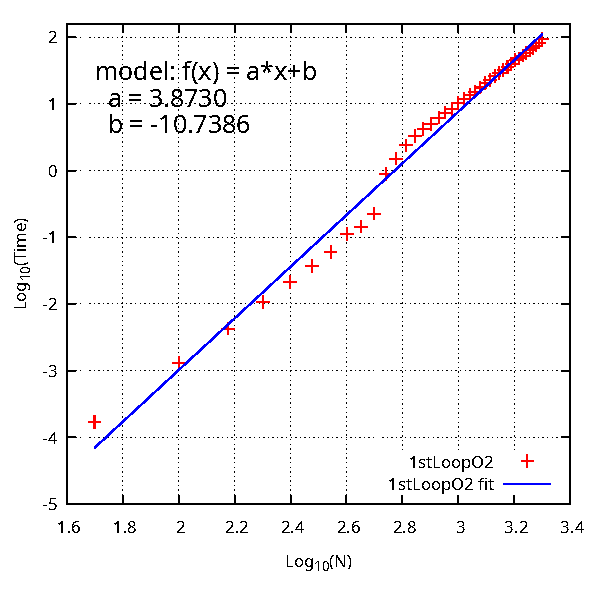
\includegraphics[width=1\linewidth]{Data/Fit_1stLoopO2}
		\caption{Fit of \textit{1stLoop} data with -O2 flag}
		\label{fig:fit1stloopo2}
	\end{subfigure}%
	\hfill
	\begin{subfigure}{0.47\textwidth}
		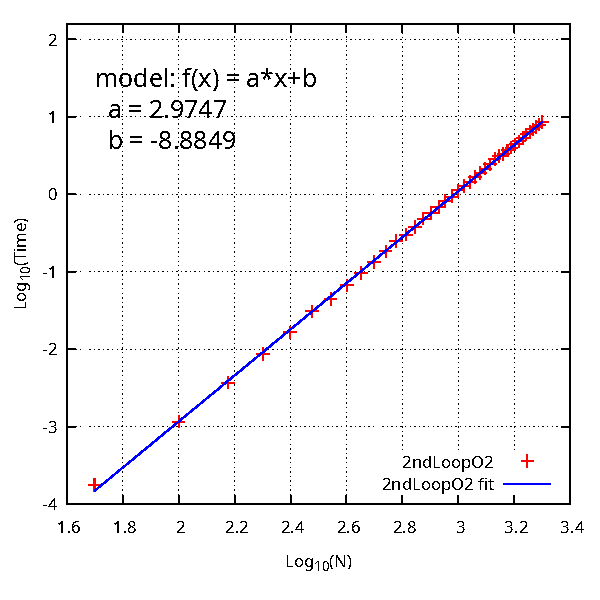
\includegraphics[width=1\linewidth]{Data/Fit_2ndLoopO2}
		\caption{Fit of \textit{2ndLoop} data with -O2 flag}
		\label{fig:fit2ndloopo2}
	\end{subfigure}
	\begin{subfigure}{0.47\textwidth}
		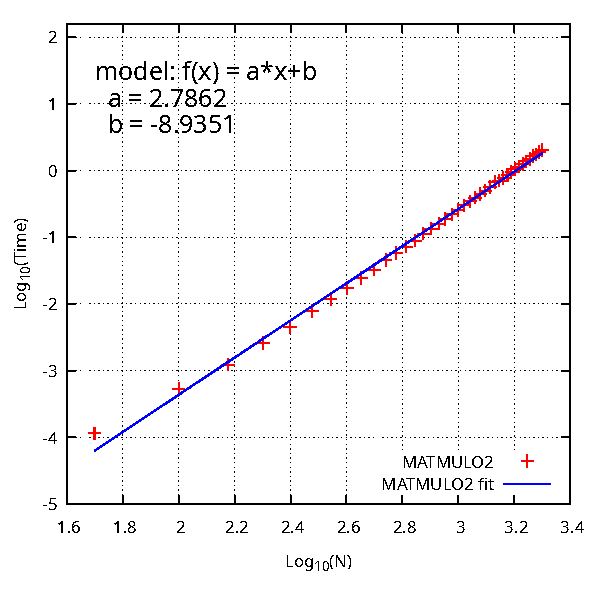
\includegraphics[width=1\linewidth]{Data/Fit_MATMULO2}
		\caption{Fit of \textit{MATMUL} data with -O2 flag}
		\label{fig:fitMATMULo2}
	\end{subfigure}
	\caption{Fitted curves for the three methods with -O2 flag.}
	\label{fig:fitso2}
\end{figure}

\newpage
\section{Self-evaluation} %What have you learned? What can be done next? What went wrong and why?

Things learned while completing this assignment are:
\begin{itemize}
	\item how to call a compiled program from a python script by using the libraries \textit{subprocess} or \textit{os.system};
	\item how to use \textit{gnuplot} interactively and also in a script.
\end{itemize}

It would have been better to run the program with a non-equally spaced sequence of values for the matrix size to have better linear fits and plots in double log scale.
Also, it could be useful also to automatize the plot of the residuals of the fits in order to check their quality and reliability.

\end{document}
